\section{Scopo e strumentazione}

Abbiamo impiegato due diversi dispositivi (un calibro utilizzato come reticolo di diffrazione ed un interferometro di Michelson) con l'obiettivo di misurare la lunghezza d'onda della luce emessa rispettivamente da un laser ad He-Ne e da una lampada al mercurio. Strumenti utilizzati sono dunque un laser ad He-Ne, un calibro ventesimale (quindi il passo è pari ad 1 mm), schermi su cui visualizzare le figure di diffrazione o di interferenza, un metro di risoluzione 1 mm e l'interferometro di Michelson, mostrato in \fig{figura_1}. Al fine di contare con maggiore efficacia le frange di interferenza nella seconda parte dell'esperienza abbiamo talvolta utilizzato anche un dispositivo di registrazione che ci ha permesso poi di eseguire il conteggio, con più calma, su uno schermo.\\
\subsection{Lunghezza d'onda di un laser He-Ne}
Abbiamo posto il laser su un tavolo in modo da avere un'emissione quasi ortogonale alla normale al tavolo stesso. Infatti solo così il passo reticolare visto dalla radiazione diviene confrontabile con la lunghezza d'onda (di circa 650 nm) ed è quindi visualizzabile la figura di diffrazione. Quest'ultima compare su uno schermo(costituito da un foglio) posto a circa 2.5 m dall'estremo del tavolo.\\
\subsection{Interferometro di Michelson}
L'interferometro è costituito da due bracci disposti a croce, ciascuno dei quali termina con degli specchi che riflettono la radiazione luminosa. Esistono due cammini ottici possibili; in uno di questi la luce procede fino allo specchio M$_2$, da cui viene riflessa per poi essere mandata dal beam splitter allo schermo. Nel secondo cammino ottico la luce è riflessa dal beam splitter su M$_1$, da cui torna all'osservatore. Lo specchio M_2 può essere soltanto orientato manovrando due viti al fine di allineare l'interferometro. Lo specchio M$_1$ può invece essere spostato agendo su un micrometro avente risoluzione di 10 $\mu$m: in tal modo può essere variato il cammino ottico e le frange circolari della figura di diffrazione scorrono, dando luogo a interferenza.

\section{Misura della lunghezza d'onda di un laser He-Ne}

Abbiamo dapprima agito sulla posizione ed orientamento del calibro, in modo che la luce incidesse sulla parte graduata. Quindi abbiamo variato l'inclinazione del fascio agendo sulla vite posta sul retro del laser, in modo da avere una figura di diffrazione evidente, con almeno 15 ordini chiaramente visualizzabili ed in modo che lo spessore delle tracce fosse il minore possibile.\\
Abbiamo allora segnato con una matita tanto la posizione del livello quanto lo spessore della traccia luminosa, ripetendo il procedimento per ciascun livello (ne abbiamo contati in totale 21), compreso l'ordine 0 di riflessione. Abbiamo anche individuato la posizione della traccia, di forma circolare come l'apertura del laser, corrispondente alla parte di segnale non deviato. Con il metro si è così potuto misurare la distanza tra il centro del cerchio e l'ordine 0, segnando a matita il punto medio tra queste due posizioni. Abbiamo allora misurato la distanza tra questo punto medio ed i due estremi della figura luminosa presente sul calibro, considerando poi media e semidispersione per ottenere la distanza tra il calibro e lo schermo pari a $D = 206.0 \pm 1.5$ $cm$. Abbiamo valutato l'errore dato dalla semidispersione prevalente sugli errori dovuti al non perfetto allineamento.

\subsection{Analisi dati}

Utilizzando il metro si è potuto misurare la distanza tra il punto medio, utilizzato come riferimento, e ciascuno dei livelli precedentemente individuati. In \tab{tabella 1} sono riportati i dati, compreso un errore, e l'ordine di diffrazione m. L'errore è ottenuto dalla somma in quadratura dell'errore dovuto allo spessore di ciascuna tacca, l'errore dovuto alla risoluzione del metro ed un errore di 5 mm corrispondente al raggio del cerchio (incertezza sulla posizione di riferimento).
%tabella 1
Essendo l'angolo di diffrazione il complementare dell'angolo di cui è nota la tangente tan$\theta$ = h/D, si ha la relazione, essendo $\theta_i$ l'angolo di incidenza rispetto alla normale, d il passo reticolare e $\lambda$ la lunghezza d'onda:
\begin{equation}
cos\theta = sen\theta_i - m \frac{\lambda}{d}
\label{legge_diffrazione}
\end{equation}
Noto quindi $cos\theta = \frac {1}{\sqrt{1+tan\theta ^2}}$, abbiamo svolto un fit lineare del coseno in funzione dell'ordine di diffrazione, mantenendo come parametri $a = -\frac{\lambda}{d}$ e $b = sen\theta_i$ e considerando come errore solo l'errore sul coseno, ottenuto dalla propagazione degli errori su h e su D. I risultati ottenuti sono i seguenti:
\begin{itemize}
\item $a = -0.000626 \pm 0.000008$
\item $b = 0.99952 \pm 0.00006$, quindi angolo di incidenza, come atteso, molto vicino a $\pi$/2
\item $cov = -0.62$ come valore di covarianza normalizzata
\item $\chi^2 = 0.07$ con 19 gradi di libertà.
\end{itemize}
Il valore del $\chi^2$ fa pensare ad una possibile sovrastima dell'errore; del resto in esso sono state inserite parti sistematiche. Noto d, si è ottenuta una lunghezza d'onda $\lambda = 626 \pm 8$ nm, pienamente compatibile con il valore atteso di 632.8 nm. Riportiamo infine in \fig{2} il grafico di $cos\theta (m)$
\begin{figure}[h]
	\centering
	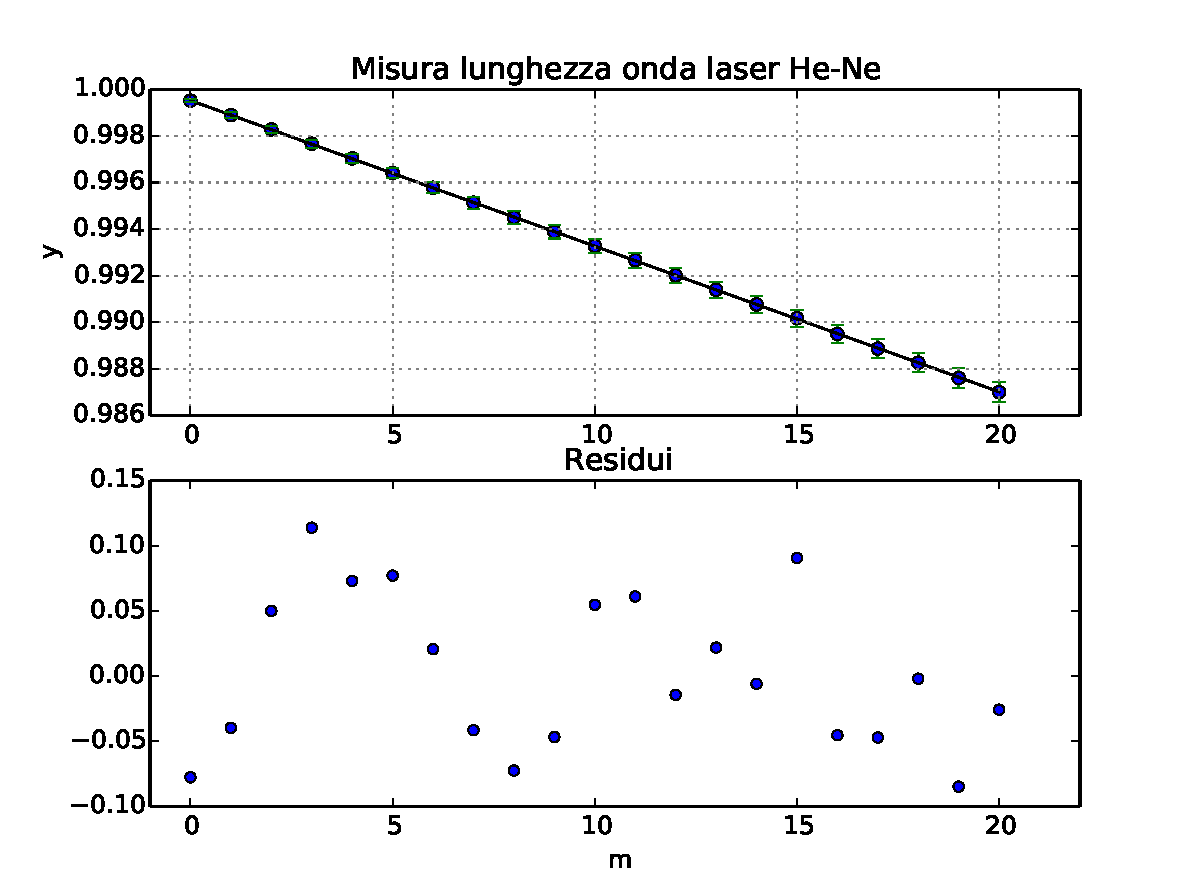
\includegraphics[scale=0.5]{grafico.pdf}
	\caption{}
	\label{f:spettroscopio_reticolo}
\end{figure}


